\chapter{Iridis Oops!} 
\label{sec:bugs}
\lstset{style=6502Style}

\section{The Byte that Broke}
The earliest editions of Iridis Alpha contained a crash bug that manifested itself
during the bonus phase. One moment, the player was barrelling their ugly vertically-oriented
gilby through the game's obstacle course; the next, the game came to an abrupt halt:

\begin{figure}[H]
    \centering
    \frame{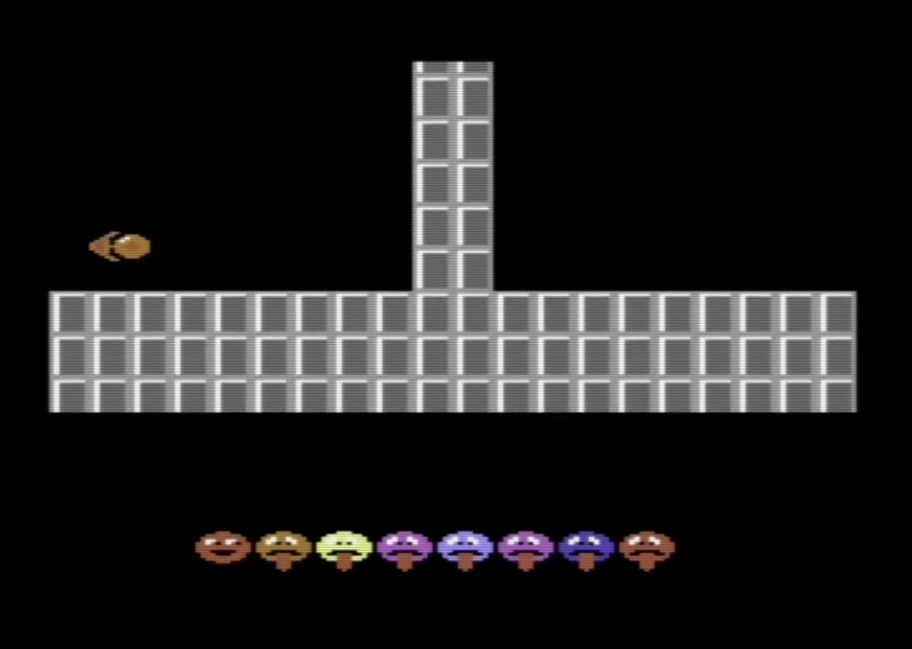
\includegraphics[width=5.5cm]{bugs/before.png}}%
    \hspace{0.5cm}
    \frame{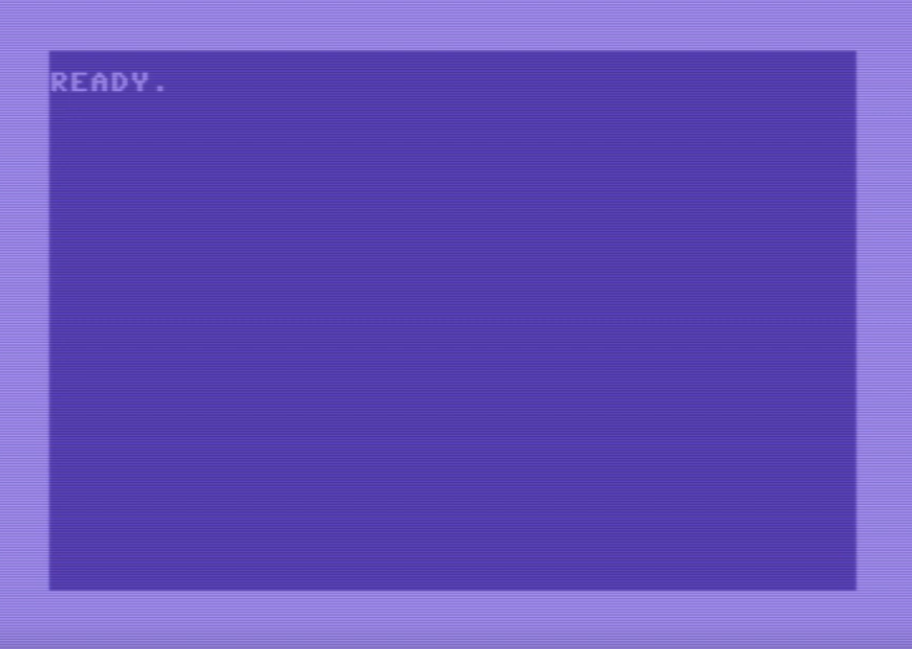
\includegraphics[width=5.5cm]{bugs/after.png}}%
\caption{You're minding your own business playing this horrible mini-game when it mercifully crashes.}
\end{figure}

Despite its incredibly rapid pace of development and release this fault was not due
to some overlooked glitch in the code of the game.

What happened is that the mastering process had dropped the very last byte in the second
section of game data on the tape. You may recall there were four chunks of data encoded on
the cassette edition of Iridis Alpha, each containing data to be stored at different points
in the C64's memory space.

\begin{definition}[Jeffrey Breaks the Bad News]
\setlength{\intextsep}{0pt}%
\setlength{\columnsep}{3pt}%
\begin{wrapfigure}{l}{0.12\textwidth}
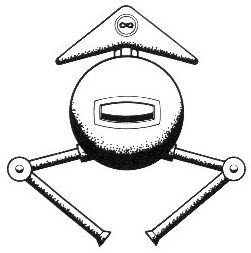
\includegraphics[width=\linewidth]{src/callout/ia.jpg} 
\end{wrapfigure}
\small
"We must apologise to some of the earliest purchasers of Iridis Alpha... it
seems that some data was corrupted during the production phase of the
data duplication, and the first few hundred copies of the game used to bug
out if you lost at the Bonus Phase. All the buggy copies known of have
been replaced, and all current tapes are fine, but if you find you have a
buggy version you should send it back to those awfully nice Hewsons
people and they ll give you an unglitchified one."
\end{definition}

The fault lay in a single byte. The very last byte in the second segment on the tape was missing
completely. Instead on \icode{\$A2} value, there was nothing. With the result that the byte
stored in the C64's memory at that position was uninitialized and remained \icode{\$00}:
\begin{figure}[H]
  {
    \setlength{\tabcolsep}{3.0pt}
    \setlength\cmidrulewidth{\heavyrulewidth} % Make cmidrule = 
    \begin{adjustbox}{width=10cm,center}

      \begin{tabular}{lllllllll}
        \toprule
        Start Address & End Address & Note & \\
        \toprule
\icode{0800} & \icode{BFFE}  & This one was fine.\\
        \icode{BF00} & \icode{BFFF}  & The last byte in this section (\icode{\$A2}) was missing.\\
\icode{C000} & \icode{CFFE}  & This one was fine.\\
\icode{E000} & \icode{F7FF}  & This one was fine.\\
        \addlinespace
        \bottomrule
      \end{tabular}

    \end{adjustbox}

  }\caption{Chunk \icode{BF00} is missing its last byte.}
\end{figure}

If we look at the data as it should have been we can see the assembly language the machine code would
have translated to. The \icode{\$A2} is an \icode{LDA} instruction that loads the value \icode{\$07} into
the \icode{A} register:
\begin{lstlisting}[caption=The data segment as it should be\, with \icode{\$A2} at \icode{\$BFFF},escapechar=\%]
Address      Bytes       Assembler
$BFFF	       A2 07       LDX #$07
$C001	       A9 08       LDA #$08
$C003	       8D F8 BF    STA $BFF8
\end{lstlisting}

However, because the value at \icode{\$BFFF} was \icode{\$00} instead of \icode{\$A2} we end up with this
invalid sequence of instructions.
\begin{lstlisting}[caption=The corrupt byte\, with \icode{\$00} at \icode{\$BFFF},escapechar=\%]
Address      Bytes       Assembler
$BFFF        00          BRK
$C000        07 A9       SLO $A9
$C002        08          PHP
$C003	       8D F8 BF	   STA $BFF8
\end{lstlisting}
The first two are probably not fatal, however \icode{PHP} pushes a value onto the stack. Once the stack is invalid
things are going to go south fast. It was probably this instruction, the last invalid one before the bytes started
to make sense again, that sunk this faulty pressing of Iridis Alpha with all hands.

\begin{figure}[H]
  {
    \begin{adjustbox}{width=14cm,center}
      \surface{bugs/spool-sections-glitches.png}
    \end{adjustbox}
  }\caption[]{The problematic section of data highlighted in red.}
\end{figure}



\section{Reappearing Enemies}

When you start a new game, enemies\index{enemies} from the previous game show up in the first
wave. For most people starting out, this will take the form of a few residual
'licker ships' zapping them just as they're getting started.

This bug happens because the 'wave' data isn't cleared down when a new game
starts. So whatever is in there from the previous game gets used until they're
flushed out by being killed and replaced with the level's proper enemy data.

This isn't a problem for the first game after Iridis Alpha is loaded because
the first level's data is hardcoded in there.

The fix is simple enough, we initialize the active wave data stored in `activeShipsWaveDataLoPtrArray\index{activeShipsWaveDataLoPtrArray}` and `activeShipsWaveDataHiPtrArray\index{activeShipsWaveDataHiPtrArray}`
with the first level's data whenever we start a new game. 

\begin{lstlisting}[caption=Fixing the reappearing enemy bug,escapechar=\%]
  LDA #$0F 
  STA $D418    ;Select Filter Mode and Volume 
  JSR ClearPlanetTextureCharsets%\index{ClearPlanetTextureCharsets}% 
  JSR InitializeActiveShipArray ; Added to fix the bug.
  JMP PrepareToLaunchIridisAlpha%\index{PrepareToLaunchIridisAlpha}% 

;------------------------------------------------------------------ 
; InitializeActiveShipArray 
;------------------------------------------------------------------ 
InitializeActiveShipArray 
  LDX #$00 
InitializeActiveShipLoop 
  LDA <planet1Level1Data%\index{planet1Level1Data}% 
  STA activeShipsWaveDataLoPtrArray%\index{activeShipsWaveDataLoPtrArray}%,X 
  LDA >planet1Level1Data%\index{planet1Level1Data}% 
  STA activeShipsWaveDataHiPtrArray%\index{activeShipsWaveDataHiPtrArray}%,X 
  INX 
  CPX #$10 
  BNE InitializeActiveShipLoop 
  RTS 
\end{lstlisting}

\section{A Sort of Cheat}

After a minute or two in the title screen\index{screen}, the game enters 'Attract Mode' and
plays a random level on autopilot for a few seconds. If you press F1 during
this play you enter the 'Made in France' pause-mode mini game. If you press F1
again you can now start playing the level 'Attract Mode' selected at random.

This is because the `CheckKeyboardInGame\index{CheckKeyboardInGame}` routine\index{routine} doesn't try to prevent you
from entering 'Pause Mode' while Attract Mode is running:

\begin{lstlisting}[caption=Fixing the reappearing enemy bug,escapechar=\%]
CheckKeyboardInGame%\index{CheckKeyboardInGame}%
        LDA lastKeyPressed%\index{lastKeyPressed}%
        CMP #$40 ; $40 means no key was pressed
        BNE KeyWasPressed%\index{KeyWasPressed}%
        LDA #$00
        STA f1WasPressed%\index{f1WasPressed}%
ReturnEarlyFromKeyboardCheck%\index{ReturnEarlyFromKeyboardCheck}%   
        RTS

KeyWasPressed%\index{KeyWasPressed}%   
        LDY f1WasPressed%\index{f1WasPressed}%
        BNE ReturnEarlyFromKeyboardCheck%\index{ReturnEarlyFromKeyboardCheck}%
        LDY attractModeCountdown%\index{attractModeCountdown}%
        BEQ b787C
        ; If a key is pressed during attract mode, accelerate the
        ; countdown%\index{countdown}% so that it exits it nearly immediately.
        LDY #$02
        STY attractModeCountdown%\index{attractModeCountdown}%
\end{lstlisting}

